% Este arquivo .tex será incluído no arquivo .tex principal. Não é preciso
% declarar nenhum cabeçalho

\section{Diversão}
Está com vontade de fazer algo para livrar a cabeça do stress da vida acadêmica?
Como em toda universidade, Na Unicamp existem inúmeras de opções de
entreterimento e diversão. Desde festas e bares até cinemas e teatros. 

Se você gosta ou se interessa por jogos de tabuleiro, a dica é a luderia que
existe na 2, o Metropoly. Lá você paga 12 Reais por pessoa e joga a vontade. A
comida e bebida são um pouco caras, mas mesmo assim compensa. Se você não sabe o
que jogar, peça sugestões aos garçons de jogos. 

O Cinema mais próximo e mais conveniente é o do Shopping Dom Pedro. Estudantes
pagam meia da meia na segunda feira, então é uma ótima opção para quem quer se
divertir sem gastar muito dinheiro.

Se você curte festas e baladas, fique atento na saída do bandeco, pois é lá que
elas são divulgadas. A maioria das festas acontecem às quintas feiras em
repúblicas ou no Campinas Hall. Existem também festas dentro da Unicamp, que
apesar de serem proibidas, acontecem com certa regularidade.

\subsection{Espaços culturais}

\begin{itemize}
    \item   \textbf{Casa do Lago:} Dentro da Unicamp, mantém uma programação
        quase diária de cinema e exposições. Este ano estão viabilizando a
        instalação de café e revistaria. A página da casa do lago é:
        \\\url{www.preac.rei.unicamp.br/casadolago}

    \item   \textbf{Semente:} Fica no fim da avenida Santa Isabel, depois da
        moradia. Sempre tem apresentações artísticas, como teatros e espetáculos
        musicais.
\end{itemize}

\subsection{Cinemas}

\begin{itemize}
    \item   \textbf{Kinoplex}
        \\Endereço: Shopping D. Pedro (Rodovia Dom Pedro I, Km 137 -- Jd. Sta. Genebra)
        \\Telefone: (19) 3131-2800
        \\Site: \url{kinoplex.com.br}

    \item   \textbf{Cinemark Iguatemi}
        \\Endereço: Shopping Center Iguatemi (Av. Iguatemi, 777 -- Vila Brandina)
        \\Site: \url{cinemark.com.br}

    \item   \textbf{Box Cinépolis Campinas}
        \\Endereço: Campinas Shopping (Rua Jacy T. de Camargo, 940 -- Jardim do Lago)
        \\Telefone: (19) 3268-2288
        \\Site: \url{cinepolis.com.br}

    \item   \textbf{Cine Galleria}
        \\Endereço: Galleria Shopping (Rod. Dom Pedro I, Km, 131,5 -- Jd. Nilópolis)
        \\Telefone: (19) 3207-1333
        \\Site: \url{www.galleria.com.br/page/cinema.asp}

    \item   \textbf{Cine Moviecom Unimart}
        \\Endereço: Shopping Unimart (Av. John Boyd Dunlop, 350 -- Chácara da República)
        \\Telefone: (19) 3744-4791
        \\Site: \url{moviecom.com.br}

    \item   \textbf{Multiplex Parque das Bandeiras}
        \\Endereço: Shopping Parque das Bandeiras (Av. John Boyd Dunlop, 3900)
        \\Telefone: (19) 3227-1869
        \\Site: \url{www.cinearaujo.com.br/salas.asp?cin_id=45}
		
    \item   \textbf{Topázio Cinemas}
        \\Endereço: Shopping Prado (Av. Washington Luís, 2480 -- Parque Prado)
        \\Telefone: (19) 3276-3610
        \\Site: \url{www.shoppingprado.com.br/web/cinema/}

    \item   \textbf{Cinesercla Spazio Ouro Verde}
        \\Endereço: Shopping Spazio Ouro Verde
        \\Telefone: (19) 3726-2000
        \\Site: \url{www.cinesercla.com.br/cinemas/detalhes/cinesercla_spazio_ouro_verde}

\end{itemize}

\subsection{Teatros}

\begin{itemize}
    \item   \textbf{Lume Teatro}
        \\Endereço:  Rua Carlos Diniz Leitão, 150 Vila Santa Isabel -- Barão Geraldo
        \\Telefone: (19) 3289-9869
        \\Site: \url{lumeteatro.com.br}

    \item   \textbf{Teatro Interno Luiz Otávio Burnier}
        \\Endereço: Centro de Convivência Cultural (Praça Imprensa Fluminense s/nº -- Cambuí)
        \\Telefone: (19) 3232-5977 / (19) 3232-4168

    \item   \textbf{Teatro de Arena}
        \\Endereço: Centro de Convivência Cultural (Praça Imprensa Fluminense s/nº -- Cambuí)
        \\Telefone: (19) 3232-5977 / (19) 3232-4168

    \item   \textbf{Teatro Carlos Maia}
        \\Endereço: Rua Cel. Quirino, 2 -- Bosque dos Jequitibás
        \\Telefone: (19) 3231-8795

    \item   \textbf{Teatro José de Castro Mendes}
        \\Endereço: Praça Corrêa de Lemos, s/nº -- Vila Industrial
        \\Telefone: (19) 3272-9359

    \item   \textbf{Auditório Beethoven (Concha Acústica)}
        \\Endereço: Av. Heitor Penteado, s/nº -- Portão 2 -- Lagoa do Taquaral
        \\Telefone: (19) 3256-9959

    \item   \textbf{Teatro de Arte e Ofício}
        \\Endereço: Rua Conselheiro Antônio Prado, 529 -- Vila Nova
        \\Telefone: (19) 3241-7217

    \item   \textbf{Teatro Dom Nery (Externato São João)}
        \\Endereço: Rua José de Alencar, 360  Centro
        \\Telefone: (19) 3231-2644

     \item   \textbf{Teatro Teresa Aguiar (Conservatório)}
         \\Endereço: Rua José de Alencar, 701 -- Centro
    %     \\Telefone: (19) 3232-9345

    \item   \textbf{Teatro da Vila Padre Anchieta}
        \\Endereço: Av. Cardeal Dom Agnelo Rossi, s/nº -- Vila Padre Anchieta
        \\Telefone: (19) 3781-0382

     \item   \textbf{Centro Cultural Evolução}
         \\Endereço: Rua Regente Feijó, 1087 -- Centro
    %     \\Telefone: (19) 3232-9959

    \item   \textbf{Teatro Amil (Antigo Teatro TIM)}
        \\Endereço: Shopping D. Pedro, Entrada das flores
        \\Telefone: (19) 3756-9890 / (19) 3756-9891
		\\Site: \url{www.conteudoteatral.com.br/teatroamil}

    \item   \textbf{Teatro Brasil Kirin}
		\\Endereço: Shopping Iguatemi (Av. Iguatemi, 777 -- Vila Brandina).
		\\Telefone: (19) 3294-3166
		\\Site: \url{www.teatrobrasilkirin.com.br}

    \item   \textbf{Teatro do SESC}
		\\Endereço: Rua Dom José I, 270 -- Bonfim (próximo à rodoviária nova)
		\\Telefone: (19) 3737-1500

    \item   \textbf{Teatro do SESI Amoreiras}
		\\Endereço: Av. das Amoreiras, 450 -- Parque Itália.
		\\Telefone: (19) 3272-3560

    \item   \textbf{Teatro SOTAC}
		\\Endereço: Rua Barão de Jaguara, 2 -- Bosque
		\\Telefone: (19) 3235-2266
		\\Site: \url{www.sotac.com.br}

    \item   \textbf{Teatro Sia Santa}
		\\Endereço: Rua Sebastião Paulino dos Santos, 20 -- Parque Santa Bárbara
		\\Telefone: (19) 3281-3306
		\\Site: \url{www.siasanta.art.br}
\end{itemize}

\subsection{Boates e baladas}

\begin{figure}[h!]
    \centering
    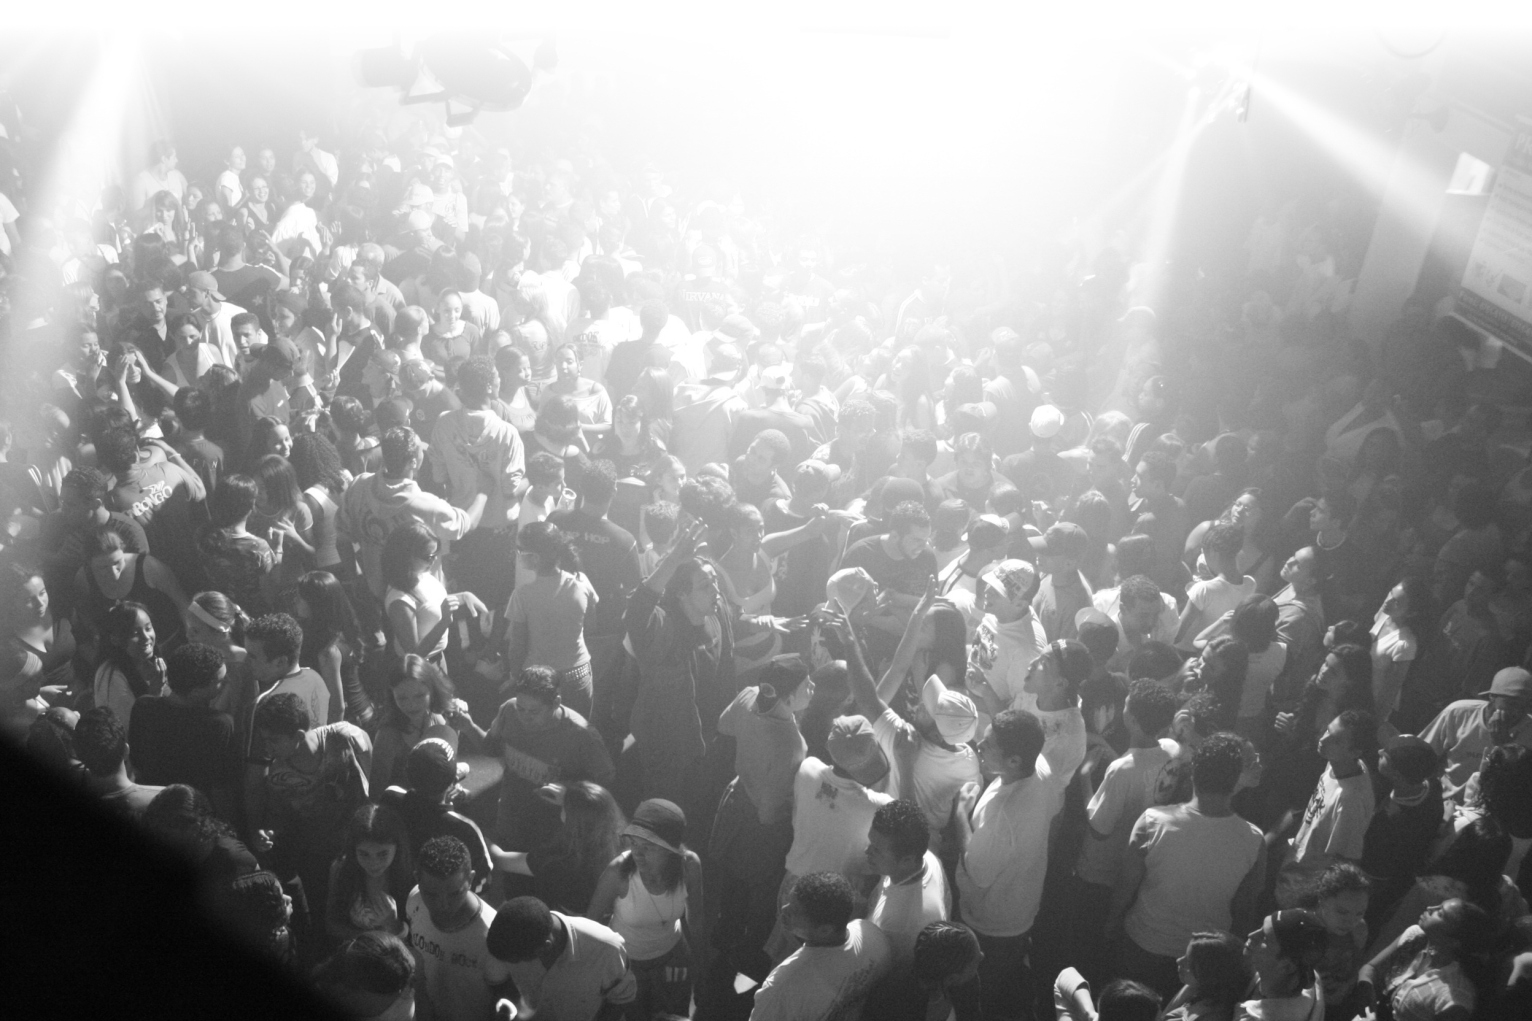
\includegraphics[width=.45\textwidth]{img/barao/boate.jpg}
\end{figure}

\begin{itemize}
    \item   \textbf{Cooperativa Brasil:} Para quem gosta de um bom forró, sempre
        com shows diversos. A galera gosta muito da quarta-universitária.
        \\Site: \url{cooperativabrasil.com.br}

    \item   \textbf{Campinas Hall:} Muitas das festas mais legais da Unicamp
        acontecem lá (como a Festa Brega e a Festa do Contrário), perto da PUCC.
        É bem grande.

    \item   \textbf{Delta Blues Bar:} O melhor do Blues \& Rock 'n Roll de
        Campinas.
        \\Site: \url{deltabluesbar.com.br}

    \item   \textbf{Swingers:} Tem bebidas caras e cada noite tem um tema, mas é
        melhor às quartas e quintas-feiras. Só homens maiores de 21 e mulheres
        com mais de 18 anos podem entrar.

    \item   \textbf{Gold:} Assim como a Swingers fica no Shopping D. Pedro.
        Balada cara, frequentada geralmente por gente mais velha.
        \\Site: \url{goldstreetbar.com.br}

    \item   \textbf{Barril da Máfia:} Programação musical bem variada e um clima
        bem legal.
        \\Site: \url{barrildamafia.com.br}

    \item   \textbf{Kraft:} Localizada próxima ao Taquaral (na Avenida
        Imperatriz Leopoldina), toca musica psi a noite toda e fica aberta até
        quase o amanhecer. Mulher entra de graça até a meia-noite.

    \item   \textbf{Cambuí:} Neste bairro existem diversos barzinhos, a maioria
        é temático, alguns são um pouco caros e cobram covert. É um ótima
        escolha para quem tiver carro pois fica um pouco longe de Barão.
\end{itemize}

\subsection{Shopping Centers}

\begin{figure}[h!]
    \centering
    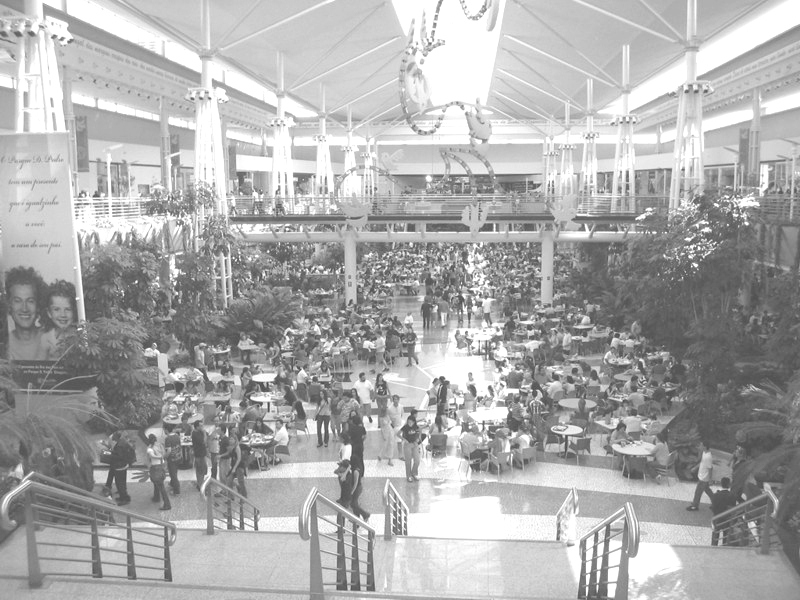
\includegraphics[width=.45\textwidth]{img/barao/d_pedro.jpg}
\end{figure}

\begin{itemize}
    \item   \textbf{Shopping Parque D. Pedro:} Foi considerado o maior shopping
        da América Latina até pouco tempo atrás. Localiza-se na Rodovia Dom
        Pedro, km 137 (razoavelmente próximo à Unicamp). O ônibus 3.38, que sai
        do Terminal Barão, vai para lá e para o Iguatemi. Outras opções de
        ônibus saindo do terminal são 2.10 e 3.00.
        \\Site: \url{parquedpedro.com.br}

    \item   \textbf{Shopping Iguatemi:} Shopping normal, o mais antigo e o
        segundo maior de Campinas. Localiza-se na Avenida Iguatemi, 777. O 3.38
        demora uns 40 minutos para chegar lá. Frequentado pela galera mais nova
        e pelo pessoal com um pouco mais de dinheiro.
        \\Site: \url{www.iguatemicampinas.com.br}

    \item   \textbf{Parque das Bandeiras Shopping:} Inaugurado no fim de 2012.
        Localiza-se na região do Campo Grande, região noroeste de Campinas 
        (MUITO longe). Conta com telas de cinema de 300 m$^{2}$.
        \\Site: \url{shoppingparquedasbandeiras.com.br}

    \item   \textbf{Shopping Jaraguá:} Shopping pequeno. Localizado na Rua Conceiçao, 
         230, no Centro de Campinas. O ônibus 3.30, no sentido Terminal Central -- Unicamp,
         para razoavelmente próximo a ele. Até 2009 existia uma outra unidade na 
         Avenida Brasil.

    \item   \textbf{Campinas Shopping:} Longe a dar com pau, mas as lojas não
        são muito caras. Localiza-se no Jardim do Lago, às margens das rodovias 
        Anhanguera e Santos Dumont. Provavelmente você nunca irá lá.
        \\Site: \url{campinasshopping.com.br}

    \item   \textbf{Shopping Prado:} Shopping pequeno, porém as lojas são um 
        pouco caras. É outro que fica muito longe e que você provavelmente nunca 
        irá até lá. Localizado na Av. Washington Luís, 2480 -- Parque Prado.
        \\Site: \url{shoppingprado.com.br}

    \item   \textbf{Galleria Shopping:} Muito bonito, mas lojas muito caras.
        Também localizado na Rodovia Dom Pedro, mas no km 131,5. O ônibus 3.00
        sai do terminal de Barão Geraldo e passa lá.
        \\Site: \url{www.galleria.com.br}

    \item   \textbf{Shopping Unimart:} Shopping pequeno, as lojas não são muito
        caras. Localiza-se na Avenida John Boyd Dunlop, 350. O ônibus 1.34 sai
        do terminal de Barão Geraldo e passa próximo.
        \\Site: \url{unimart.com.br}
    
    \item   \textbf{Shopping Spazio Ouro Verde:} Shopping pequeno, inaugurado 
        no fim de 2010. As lojas não são muito caras. É outro Shopping que 
        também fica MUITO longe. Localiza-se na Av. Ruy Rodriguez, 3900, 
        Parque Universitário (região do Ouro Verde).
        \\Site: \url{spazioouroverde.com.br}

    \item   \textbf{Ventura Mall:} Shopping pequeno, porém as lojas são muito caras.
        Fica localizado na Av. Moraes Salles, 2790 -- Nova Campinas.
        \\Site: \url{venturamall.com.br}
\end{itemize}
